\documentclass[11pt]{article}
\usepackage[margin=1in]{geometry}
\usepackage{amsmath,amssymb,amsthm}
\usepackage{graphicx}
\usepackage[hidelinks]{hyperref}

\newtheorem{theorem}{Theorem}
\newtheorem{lemma}{Lemma}
\newtheorem{remark}{Remark}

\newcommand{\C}{\mathbb C}
\newcommand{\R}{\mathbb R}
\newcommand{\Hh}{H_A}
\newcommand{\domA}{\operatorname{dom}A}
\newcommand{\ran}{\operatorname{ran}}
\newcommand{\norm}[1]{\left\lVert#1\right\rVert}

\title{Boundedness of the Auxiliary Operators in the\\
Generalized Krein--von Neumann Construction}
\author{Run \texttt{fa\_banach\_001}, lane 8}
\date{August 11, 2026}

\begin{document}
\maketitle

\section*{Status and source question}

\noindent\textbf{Status:} candidate full solution, likely valid; human review
requested.

Tarcsay and Titkos consider a subpositive operator
\(A:\domA\to F\) on a weak-star sequentially complete anti-dual pair
\(\langle F,E\rangle\).  Under the hypotheses of their Theorem~3.3, two
weakly continuous maps \(B,C:E\to E\) leave \(\domA\) invariant, the spectrum
of \(BC|_{\domA}\) is bounded, and
\[
 C^*A\subset AB,\qquad B^*A\subset AC.
\]
The source theorem and the definitions of its auxiliary operators are shown
below \cite{TT}.

\begin{center}
  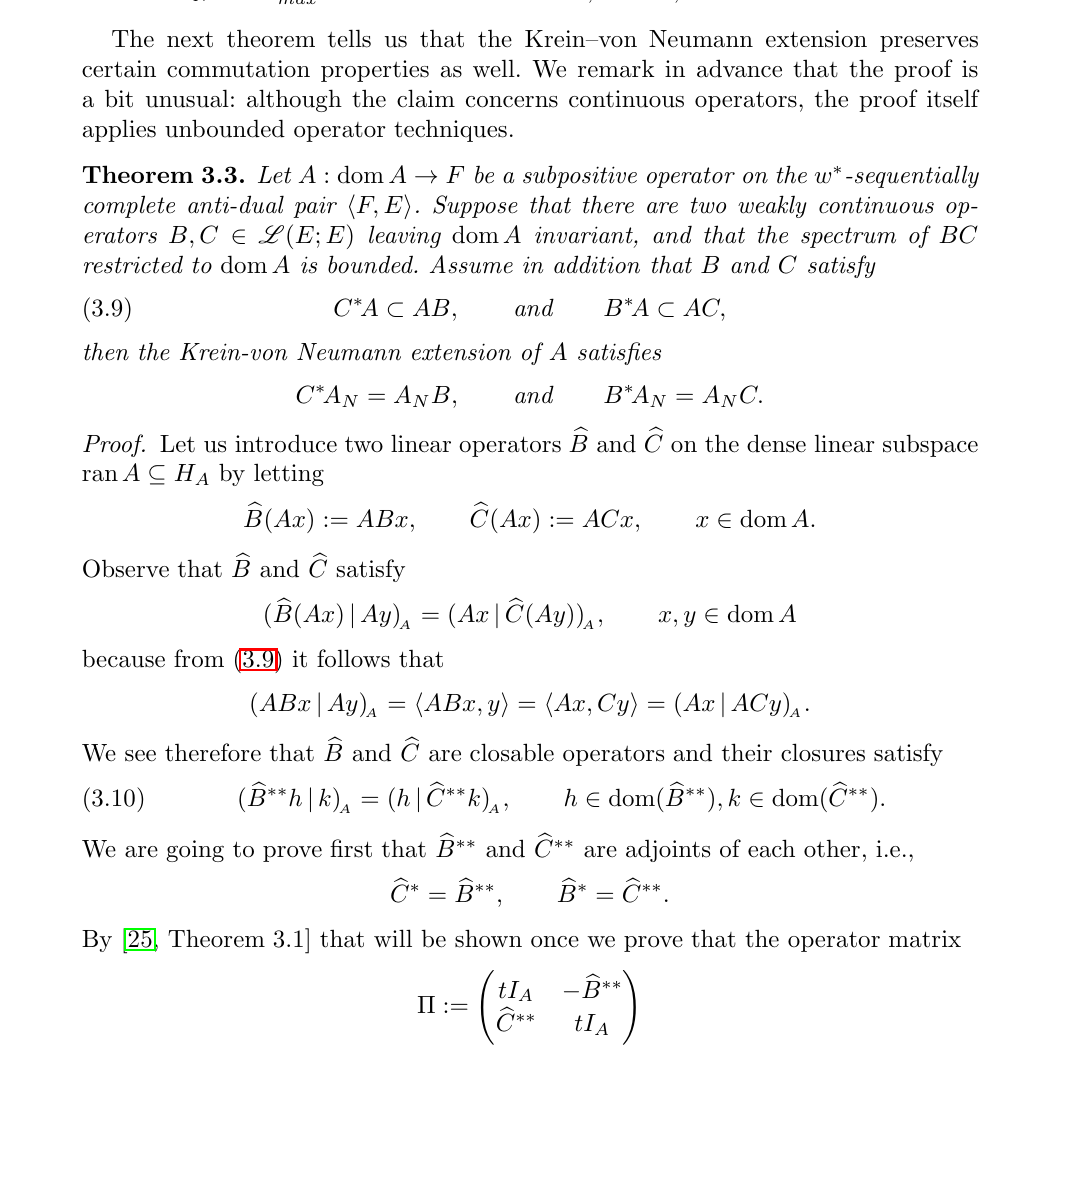
\includegraphics[width=.93\textwidth,height=.52\textheight,keepaspectratio]
  {figures/theorem_hypotheses_crop.png}
\end{center}

The auxiliary Hilbert space \(\Hh\) is the completion of \(\ran A\) for
\[
 (Ax\mid Ay)_A=\langle Ax,y\rangle,
 \qquad x,y\in\domA,
\]
and the densely defined auxiliary operators are
\begin{equation}\label{eq:aux}
 \widehat B(Ax)=ABx,\qquad
 \widehat C(Ax)=ACx.
\end{equation}
The source proves that their closures are mutual adjoints:
\begin{equation}\label{eq:source-adjoints}
 \widehat C^*=\widehat B^{**},\qquad
 \widehat B^*=\widehat C^{**}.
\end{equation}
It then explicitly leaves their boundedness open outside the Banach-space
specialization.

\begin{center}
  
\includegraphics[width=\textwidth,height=.43\textheight,keepaspectratio]
  {figures/open_question_crop.png}
\end{center}

Thus the exact source question is whether \(\widehat B,\widehat C\), more
precisely their closures, are bounded in the full anti-dual-pair setting.
The paragraph also records the expected Banach-space bound
\(\sqrt{r(BC)}\).

\section*{Idea of the proof}

Put \(T=\widehat B^{**}\).  The source identity
\eqref{eq:source-adjoints} makes \(T^*=\widehat C^{**}\), so
\(Q=TT^*\) is a positive self-adjoint operator.  On the dense subspace
\(\ran A\), this product is precisely the operator induced by \(BC\).

If \(\lambda\) lies above the bounded algebraic spectrum of
\(BC|_{\domA}\), then \(\lambda-BC\) is onto \(\domA\).  After applying \(A\),
this says
\[
 \ran A\subseteq\ran(\lambda-Q).
\]
For a self-adjoint operator, membership of a vector \(y\) in this range makes
the inverse-square potential of its spectral measure finite at \(\lambda\).
This happens at \emph{every} real \(\lambda\) above the spectral radius.

The key elementary lemma says that a finite measure on the real line cannot
have finite inverse-square potential at every point of an interval unless it
vanishes on that interval.  Applying it to the spectral measures of a dense
set kills the spectral projection of \(Q\) above the radius.  Thus \(Q\) is
bounded, which forces \(T\) and \(T^*\) bounded with the desired square-root
bound.

\section*{Inverse-square measure lemma}

\begin{lemma}\label{lem:measure}
Let \(\mu\) be a finite positive Borel measure on \(\R\), and let
\(I\subseteq\R\) be an open interval.  If
\begin{equation}\label{eq:potential}
 \int_{\R}\frac{d\mu(t)}{|t-\lambda|^2}<\infty
 \qquad\text{for every }\lambda\in I,
\end{equation}
then \(\mu(I)=0\).
\end{lemma}

\begin{proof}
Fix a compact interval \(K=[a,b]\subset I\).  For each \(\lambda\in K\),
\eqref{eq:potential} first implies \(\mu(\{\lambda\})=0\), and then
\begin{align}
 \frac{\mu((\lambda-h,\lambda+h))}{h^2}
 &\le
 \int_{0<|t-\lambda|<h}\frac{d\mu(t)}{|t-\lambda|^2}
 \longrightarrow0
 \qquad(h\downarrow0).                                      \label{eq:density}
\end{align}
The convergence follows by absolute continuity of the integral of the
integrable function \(|t-\lambda|^{-2}\).

For \(m\ge1\), let \(E_m\) consist of the points \(\lambda\in K\) for which
\[
 \mu((\lambda-h,\lambda+h))\le h^2
 \qquad(0<h<1/m).
\]
Equation~\eqref{eq:density} gives \(K=\bigcup_{m\ge1}E_m\).  We show that each
\(E_m\) has zero outer \(\mu\)-measure.  Fix
\(0<\delta<1/(5m)\).  The one-dimensional \(5r\)-covering lemma
\cite[Chapter~2]{Mattila} supplies
pairwise disjoint intervals
\[
 B_j=(\lambda_j-r_j,\lambda_j+r_j),
 \qquad \lambda_j\in E_m,\quad r_j<\delta,
\]
such that \(E_m\subseteq\bigcup_j5B_j\).  The defining estimate for \(E_m\)
applied at radius \(5r_j\) gives
\[
 \mu^*(E_m)
 \le\sum_j\mu(5B_j)
 \le25\sum_jr_j^2
 \le25\delta\sum_jr_j.
\]
The disjoint intervals \(B_j\) lie in
\([a-\delta,b+\delta]\), hence
\[
 \sum_jr_j\le\frac{b-a+2\delta}{2}.
\]
Letting \(\delta\downarrow0\) proves \(\mu^*(E_m)=0\).  Therefore
\(\mu(K)=0\), and exhaustion of \(I\) by compact intervals completes the
proof.
\end{proof}

\section*{Full boundedness theorem}

\begin{theorem}\label{thm:main}
Assume all the hypotheses of Theorem~3.3 of Tarcsay--Titkos described above.
Let
\[
 S=BC|_{\domA}:\domA\to\domA,
\qquad
 \rho=\sup\{|\zeta|:\zeta\in\sigma(S)\}<\infty,
\]
where \(\rho=0\) if \(\sigma(S)=\varnothing\).  Then the two auxiliary
operators in \eqref{eq:aux} have bounded everywhere-defined closures, and
\begin{equation}\label{eq:bound}
 \boxed{\quad
 \norm{\widehat B^{**}}
 =\norm{\widehat C^{**}}
 \le\sqrt{\rho}.
 \quad}
\end{equation}
\end{theorem}

\begin{proof}
Set
\[
 D=\ran A\subseteq\Hh,\qquad
 T=\widehat B^{**}.
\]
The subspace \(D\) is dense by the construction of \(\Hh\).  By
\eqref{eq:source-adjoints},
\[
 T^*=\widehat B^*=\widehat C^{**}.
\]
In particular, \(T\) is a closed densely defined operator.  The standard
von Neumann product theorem therefore says that
\begin{equation}\label{eq:Q}
 Q:=TT^*
\end{equation}
is a nonnegative self-adjoint operator on \(\Hh\)
\cite[Chapter~VIII]{RS}.

Both initial auxiliary operators leave \(D\) invariant.  Hence
\(D\subseteq\operatorname{dom}Q\), and for \(x\in\domA\),
\begin{equation}\label{eq:restriction}
 Q(Ax)
 =T\widehat C(Ax)
 =\widehat B\widehat C(Ax)
 =A(BC)x.
\end{equation}
No injectivity of \(A\) is used here.

Fix a real number \(\lambda>\rho\).  Then
\(\lambda I-S:\domA\to\domA\) is bijective by the definition of the
algebraic spectrum used in the source; only surjectivity will be needed.
Given \(y=Az\in D\), choose \(x\in\domA\) such that
\[
 (\lambda I-BC)x=z.
\]
Equation~\eqref{eq:restriction} gives
\begin{equation}\label{eq:range}
 y=(\lambda I-Q)Ax.
\end{equation}
Thus
\[
 D\subseteq\ran(\lambda I-Q)
 \qquad\text{for every real }\lambda>\rho.
\]

Let \(E_Q\) be the projection-valued spectral measure of \(Q\).  For
\(y\in\Hh\), write
\[
 \mu_y(\Delta)=\norm{E_Q(\Delta)y}^2
 \qquad(\Delta\subseteq\R\ \text{Borel}).
\]
If \(y\in D\), \eqref{eq:range} supplies \(u=Ax\in\operatorname{dom}Q\)
with \(y=(\lambda-Q)u\).  The spectral theorem gives
\[
 d\mu_y(t)=|\lambda-t|^2\,d\mu_u(t).
\]
In particular, \(\mu_y(\{\lambda\})=0\) and
\begin{equation}\label{eq:inverse-square}
 \int_{\R}\frac{d\mu_y(t)}{|t-\lambda|^2}
 =\mu_u(\R\setminus\{\lambda\})
 \le\norm{u}^2<\infty.
\end{equation}
This is valid for every \(\lambda\in(\rho,\infty)\).  Lemma~\ref{lem:measure}
therefore yields
\[
 \mu_y((\rho,\infty))=0,
 \qquad y\in D.
\]
Equivalently,
\[
 E_Q((\rho,\infty))y=0,\qquad y\in D.
\]
Since \(D\) is dense and a spectral projection is bounded,
\begin{equation}\label{eq:projection-zero}
 E_Q((\rho,\infty))=0.
\end{equation}

The operator \(Q\) is nonnegative.  Equation~\eqref{eq:projection-zero}
therefore confines its spectral measure to \([0,\rho]\).  The spectral
theorem now makes \(Q\) bounded and everywhere defined, with
\[
 0\le Q\le\rho I.
\]
Because \(Q=TT^*\), its domain being all of \(\Hh\) implies in particular
\(\operatorname{dom}T^*=\Hh\).  For every \(h\in\Hh\),
\[
 \norm{T^*h}^2
 =(TT^*h\mid h)_A
 =(Qh\mid h)_A
 \le\rho\norm h^2.
\]
Thus \(T^*\) is bounded by \(\sqrt\rho\).  Its adjoint
\(T=(T^*)^*\) is bounded with the same norm.  Recalling the definitions of
\(T,T^*\) proves \eqref{eq:bound}.

If \(\sigma(S)=\varnothing\), the same argument applies for every
\(\lambda>0\), so \eqref{eq:projection-zero} holds with \(\rho=0\) and
\(Q=0\).  This verifies the stated convention and completes the proof.
\end{proof}

\section*{Verification and stress tests}

The proof is analytic and uses no computation.  Six focused audits were
performed before promotion.

\begin{enumerate}
 \item The quotient issue caused by a possible kernel of \(A\) disappears in
 \eqref{eq:range}: one solves in \(\domA\) and then applies \(A\).  No induced
 inverse is assumed.
 \item The product aligned with \(BC\) is \(TT^*\), not \(T^*T\), as the
 order in \eqref{eq:restriction} confirms.
 \item The source proves the mutual-adjoint identities under exactly the
 standing bounded-spectrum hypothesis, so \(TT^*\) is legitimately
 self-adjoint.
 \item A possible spectral atom at \(\lambda\) is automatically annihilated
 in \(d\mu_{(\lambda-Q)u}=|\lambda-t|^2d\mu_u\).
 \item Lemma~\ref{lem:measure} uses pointwise finite potential and a covering
 argument, so it also rules out singular Cantor-type measures; it is not an
 unjustified absolute-continuity argument.
 \item Bounded spectral support is invoked only after \(Q\) is known
 self-adjoint.  At that point the spectral theorem makes its domain all of
 \(\Hh\), which then forces \(T^*\) everywhere defined.
\end{enumerate}

The script \path{code/crop_open_problem.py} reproducibly creates the two source
crops from pages rendered at \(180\) dpi.  It is evidence preparation, not a
proof verifier.

\section*{Scope, novelty, and human review}

Theorem~\ref{thm:main} fully answers the source's boundedness question under
the hypotheses in which the auxiliary pair was introduced, and recovers the
same spectral-radius bound previously recorded only in the Banach setting.  It
does not remove Theorem~3.3's assumption that
\(\sigma(BC|_{\domA})\) is bounded, nor does it put a norm on the ambient
anti-dual-pair spaces.

A bounded search through August 11, 2026 covered the run's four lightweight
indexes, the local arXiv source corpus, the final 2021 journal version, and
official-arXiv queries using the identifier, exact title and open sentence,
author names, auxiliary operators, anti-dual pairs, boundedness, and spectral
radius of \(BC\).  The final journal version still states the question as
open, and no later explicit answer was found.  This is not a priority claim.

Human review should focus on \eqref{eq:restriction}, the use of source
resolvent surjectivity in \eqref{eq:range}, and the outer-measure version of
the \(5r\)-covering argument in Lemma~\ref{lem:measure}.  The empty-spectrum
edge case should also be checked.

\begin{thebibliography}{9}
\bibitem{TT}
Zs. Tarcsay and T. Titkos,
\emph{Operators on anti-dual pairs: Generalized Krein--von Neumann extension},
Math. Nachr. \textbf{294} (2021), no.~9, 1821--1838;
arXiv:1810.02619.  Especially Theorem~3.3 and the following paragraph.

\bibitem{RS}
M. Reed and B. Simon,
\emph{Methods of Modern Mathematical Physics, Vol. I: Functional Analysis},
revised and enlarged edition, Academic Press, 1980.

\bibitem{Mattila}
P. Mattila,
\emph{Geometry of Sets and Measures in Euclidean Spaces},
Cambridge Studies in Advanced Mathematics 44, Cambridge University Press,
1995.
\end{thebibliography}

\end{document}
